\section{Homework 3}

\subsection{问题1}

剪枝后的与或树如图\ref{fig:3-1}所示, 共有$4$个叶子节点被剪枝.

\begin{figure*}[htbp]
    \centering
    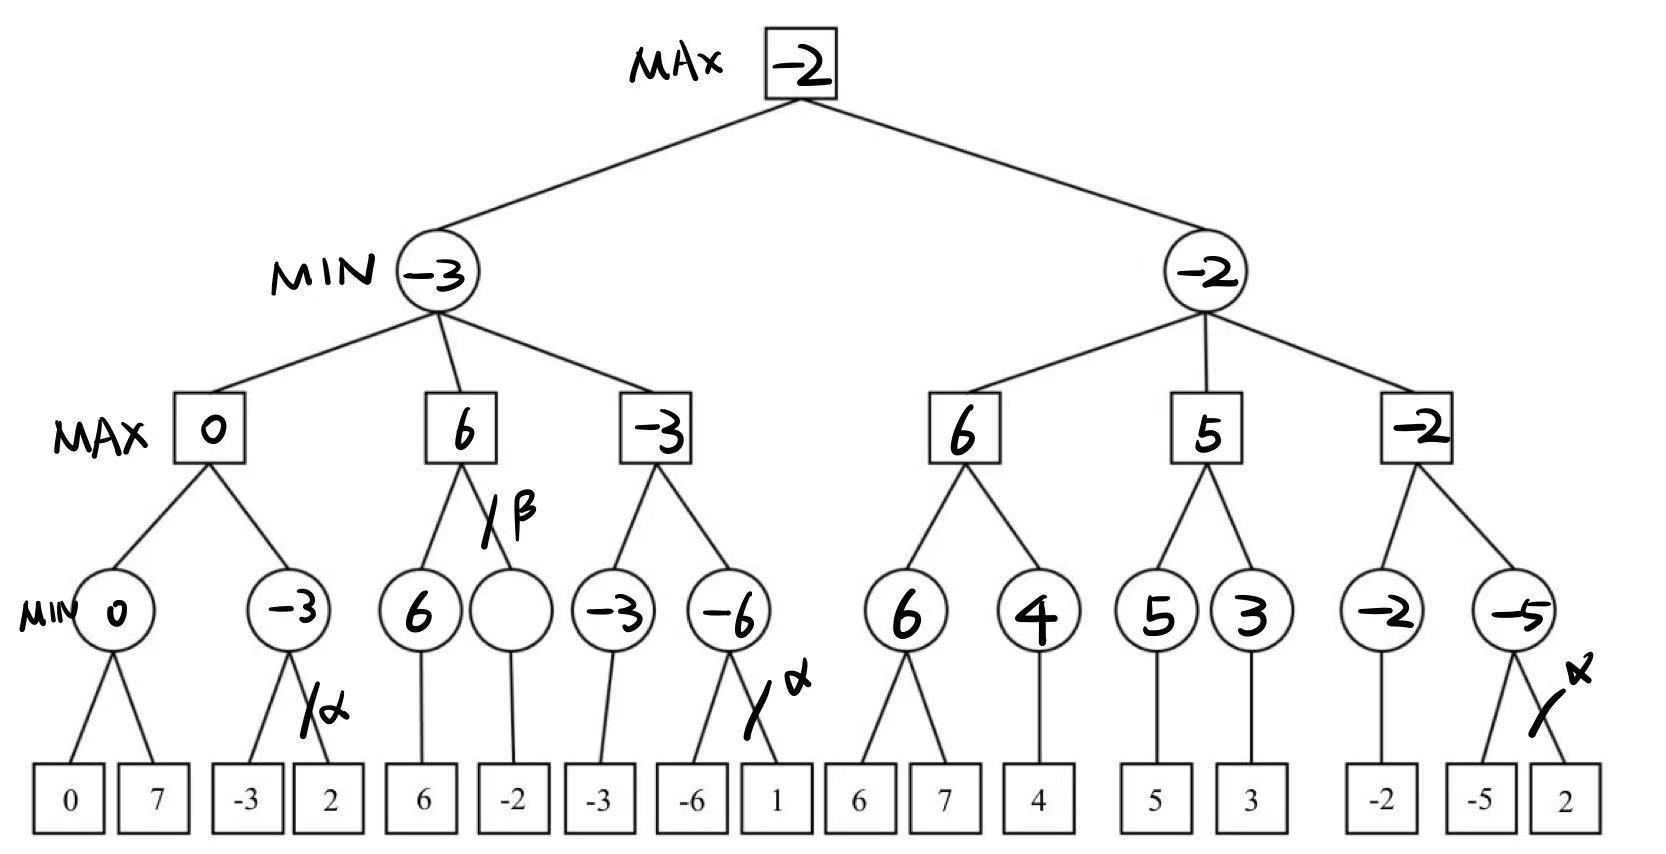
\includegraphics[width=0.7\textwidth]{images/3-1.jpg}
    \caption{3-1剪枝后决策树}\label{fig:3-1}
\end{figure*}

\subsection{问题2}

(a)用剩余石子数表示游戏的状态, 石子数为$0$则游戏结束, 若石子数为$0$时停在MIN层, 则己方赢, 记此时估值为$1$, 
MAX层的$0$为对手赢, 记估值为$0$. 则生成的博弈树如图\ref{fig:3-2(1)}所示.

\begin{figure*}[htbp]
    \centering
    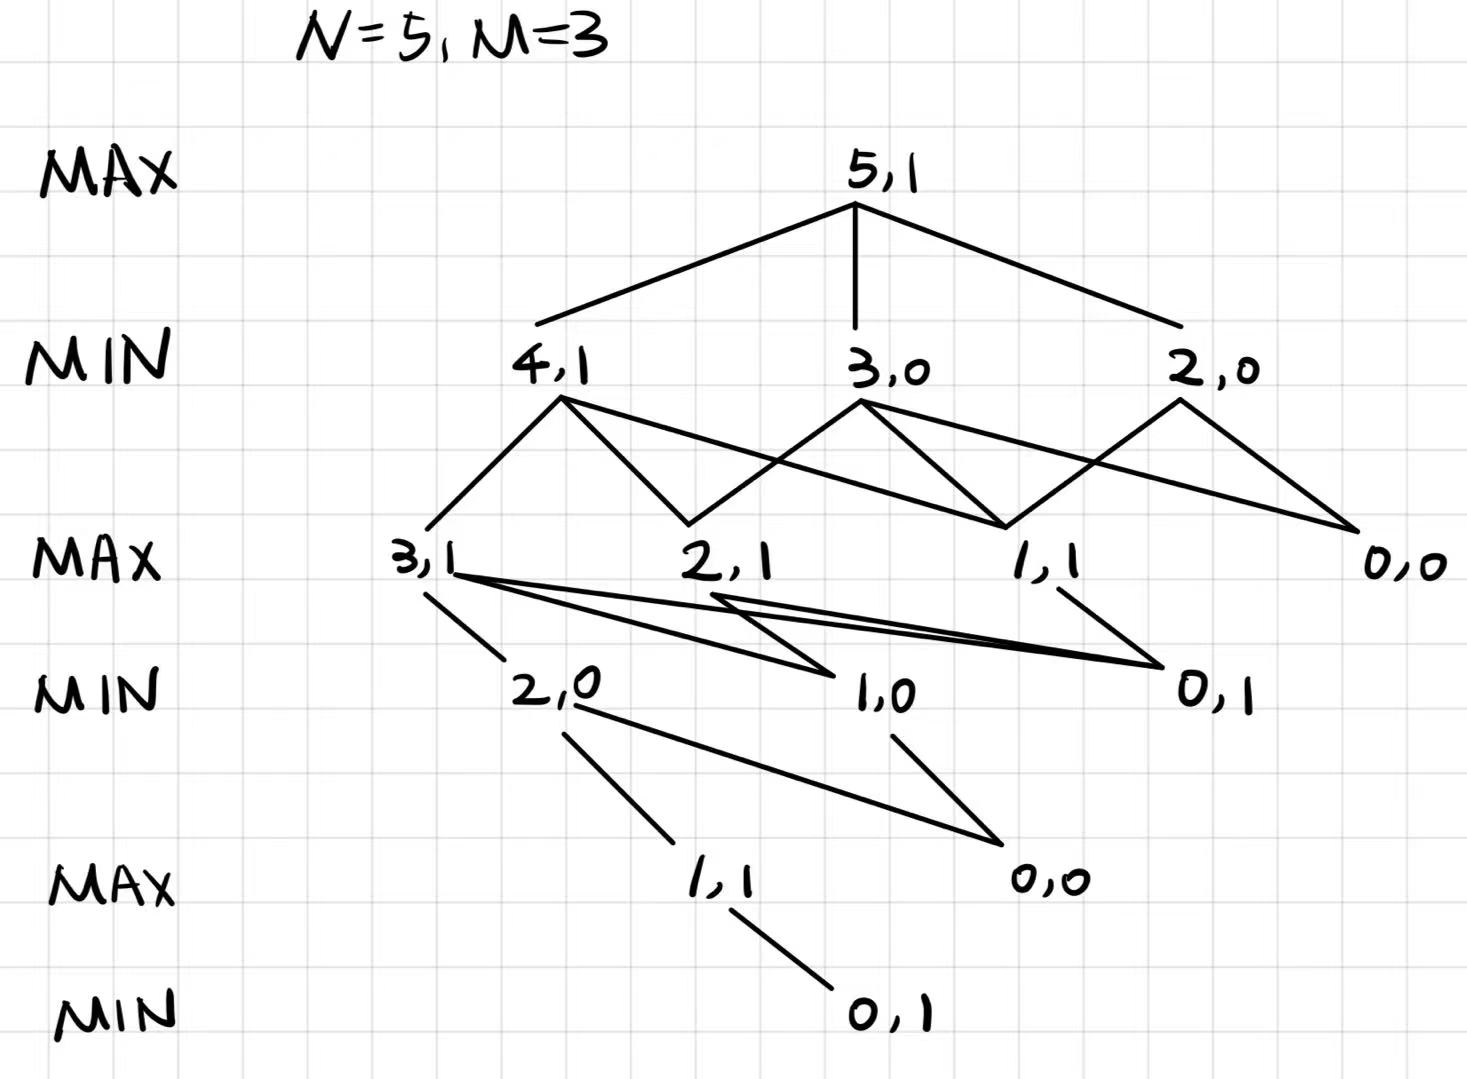
\includegraphics[width=0.7\textwidth]{images/3-2(1).jpg}
    \caption{3-2博弈树}\label{fig:3-2(1)}
\end{figure*}

(b) 由于节点估值只取$0$, $1$, 则对于MIN层节点, 若发现子节点为$0$, 则可直接进行$\beta$剪枝; 对于MAX层节点, 
若发现子节点为$1$, 则可直接进行$\alpha$剪枝. 以$N=5,M=3$的情况为例, 剪枝后的博弈树如图\ref{fig:3-2(2)}.

\begin{figure*}[htbp]
    \centering
    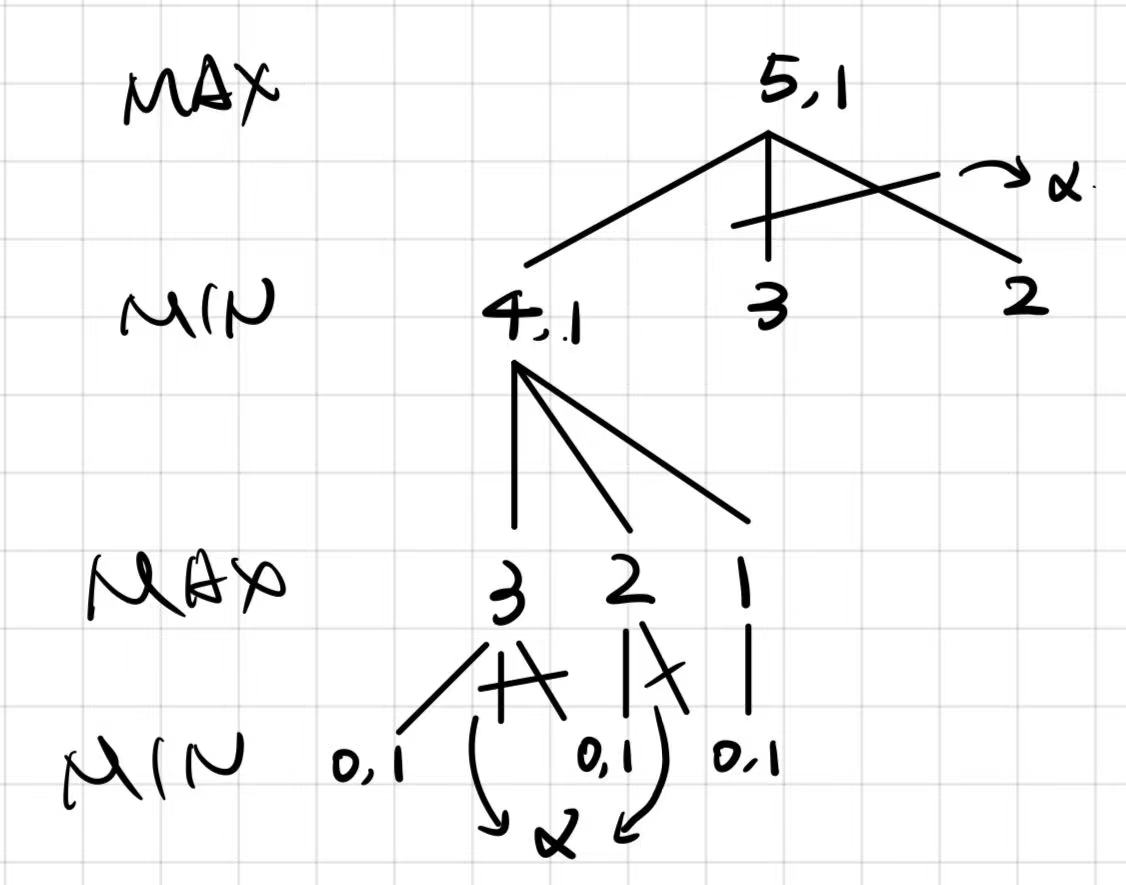
\includegraphics[width=0.7\textwidth]{images/3-2(2).jpg}
    \caption{3-2剪枝博弈树}\label{fig:3-2(2)}
\end{figure*}